\documentclass{article}
\usepackage{graphicx}
\usepackage{listings}
\usepackage{amsmath}
\usepackage{amssymb}
\usepackage{geometry}
\usepackage[colorlinks=true, linkcolor=blue, urlcolor=cyan]{hyperref}
\usepackage{bookmark} % bookmarks for PDF
\usepackage{titling}  % allows subtitle
\usepackage{tcolorbox}  % load package
\usepackage{caption} % Add this in your preamble
\usepackage{tikz} % for the border on the title page
\usepackage{fancyhdr} % for header and footer

\geometry{a4paper, margin=1in}

\newtcolorbox{notebox}{colback=green!10!white,colframe=green!50!black,title=Note,fonttitle=\bfseries}
\newtcolorbox{methodbox}{colback=purple!10!white,colframe=purple!70!black,title=Method,fonttitle=\bfseries}
\newtcolorbox{examplebox}{colback=blue!10!white,colframe=blue!70!black,title=Example,fonttitle=\bfseries}

\title{COS 122: Operating Systems}
\author{Mogale Lebethe}
\newcommand{\subtitle}{Open Notes} % <-- subtitle

% Redefine \maketitle to include subtitle
\pretitle{\begin{center}\LARGE\bfseries}
\posttitle{\par\Large\subtitle\par\vskip 0.5em\end{center}}
\preauthor{\begin{center}}
\postauthor{\par\end{center}}
\predate{\begin{center}}
\postdate{\par\end{center}}
\setlength{\parindent}{0pt}  % no paragraph indentation

\begin{document}
\begin{titlepage}
    \begin{tikzpicture}[remember picture,overlay]
        \draw[line width=1pt]
            ([xshift=1in,yshift=-1in]current page.north west) rectangle
            ([xshift=-1in,yshift=1in]current page.south east);
    \end{tikzpicture}

    \vspace*{4cm}

    \begin{center}
        {\Huge \bfseries WTW 124}\\[0.5cm]
        {\Huge \bfseries Mathematics}\\[1.5cm]
        
        \rule{\textwidth}{0.4pt}\\[1.5cm]

    
        {\normalsize \textit{Open Course Notes}}\\[1.5cm]
        {\normalsize Based on \textit{\textbf{Mathematics 124 Course Notes}}}\\[3cm]

        % Add the link here
        {\footnotesize Available at \url{https://tinyurl.com/wtw124-git}}
    \end{center}
\end{titlepage}

\tableofcontents
\newpage


\tableofcontents


\newpage

\section*{\underline{PART I: BACKGROUND}}
\phantomsection
\addcontentsline{toc}{section}{PART I: BACKGROUND}
\bookmark[page=\thepage,level=1]{PART I: BACKGROUND}

\subsection*{Chapter 1: Computer System Overview}
\phantomsection
\addcontentsline{toc}{subsection}{Chapter 1: Computer System Overview}
\bookmark[page=\thepage,level=2]{Chapter 1: Computer System Overview}

\subsubsection*{Unit 1.1: Basic Elements of a Computer System}
\phantomsection
\addcontentsline{toc}{subsubsection}{Unit 1.1: Basic Elements of a Computer System}
\bookmark[page=\thepage,level=3]{Basic Elements of a Computer System}

A computer, at a top level, consists of processor, memory, and input/output (I/O) components, with
one or more modules of each type. These components are interconnected in a certain way to allow the computer
to function as a machine that can execute programs. There are four main elements:

\begin{itemize}
    \item \textbf{Processor:} Controls the operation of the computer and performs its data processing functions. When a 
    single processor is used, it is often referred to as the \textit{central processing unit (CPU)}.
    \item \textbf{Main memory:} Stores data and programs. The memory is generally volatile, meaning that when the computer is
    turned off, the contents of memory are lost. It is also referred to as \textit{primary memory} or \textit{real memory}.
    \item \textbf{I/O modules:} Provide the means for the computer to communicate with the external environment, which may 
    consist of secondary memory (e.g. hard disks), communication equipment (e.g. keyboard, printer), terminals.
    \item \textbf{System bus:} Provides a communication path for the various components of the computer system.
\end{itemize}
\begin{figure}[!h]
    \centering
    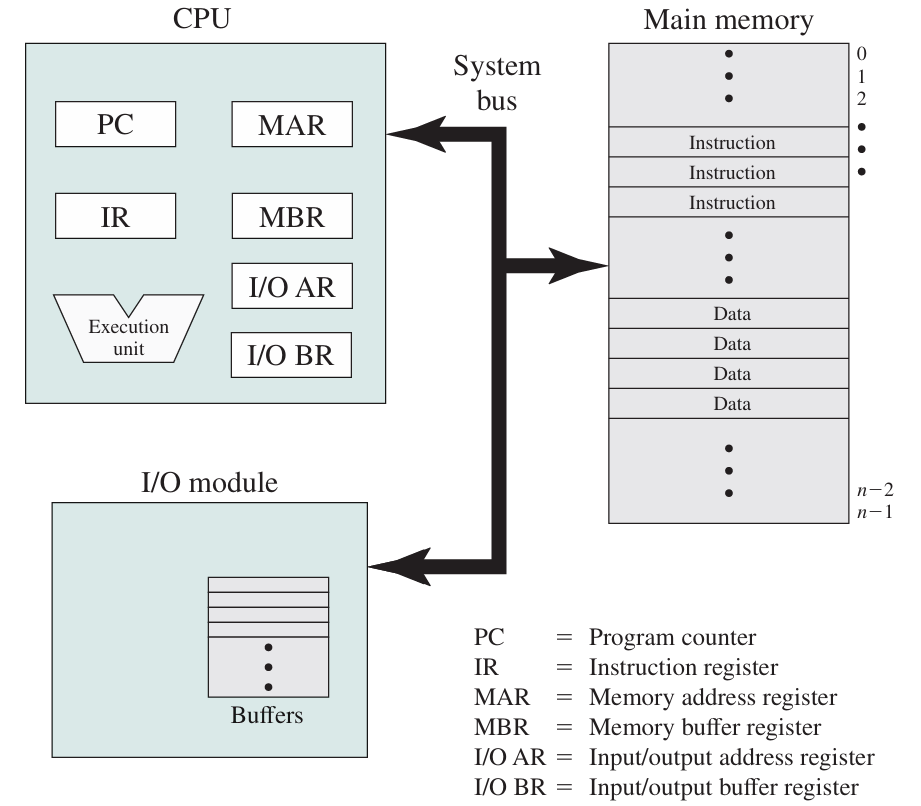
\includegraphics[width=0.7\textwidth]{figures/Ch01Figure1.png} % path to your figure
    \caption{\textbf{Computer Components: Top-Level View}}
    \label{fig:Ch01Fig1}
\end{figure}

One of the most important functions of the processor is to exchange data with the memory.
For this purpose, the processor contains two internal registers: the \textit{memory address register (MAR)} and the
\textit{memory buffer register (MBR)}. The MAR contains the address of the memory location to be accessed. The MBR
contains the data to be written into the memory or the data received from the memory.

In addition to the MAR and MBR, the processor contains a number of other registers:
\begin{itemize}
    \item \textbf{Program counter (PC):} Contains the address of the next instruction to be executed.
    \item \textbf{Instruction register (IR):} Contains the instruction currently being executed.
    \item \textbf{I/O address register (I/O AR):} Contains the address of the I/O module to be accessed.
    \item \textbf{I/O buffer register (I/O BR):} Contains the data to be written into the I/O module or the data received from the I/O module.
\end{itemize}

\begin{notebox}
    \textbf{The buffer or the address register?}

    Be careful with the terminology. The term \textit{buffer} is used for registers that hold data, while the term \textit{address register} is used for registers that hold addresses.
\end{notebox}

Figure \ref{fig:Ch01Fig1} shows the internal organisation of the processor and its connection to the memory and I/O modules.
A memory module is a set of locations, defined by sequential addresses. Each location stores a fixed number of bits, called a \textit{word}.
A word can represent data or an instruction. The number of bits in a word is called the \textit{word length} of the computer.
An I/O module transfers data between the external device, processor, and memory. It contains internal buffers to temporarily hold data being transferred.

\subsubsection*{Unit 1.2: Evolution of the Microprocessor}
\phantomsection
\addcontentsline{toc}{subsubsection}{Unit 1.2: Evolution of the Microprocessor}
\bookmark[page=\thepage,level=3]{Evolution of the Microprocessor}

The invention of the microprocessor—a processor on a single chip—sparked the desktop and handheld computing revolution. 
Modern microprocessors often have multiple cores and logical processors, while GPUs provide efficient parallel computation beyond graphics. 
CPUs now include powerful vector units, and specialised processors like DSPs handle audio, video, and other streaming signals. 
In handheld devices, the trend is toward System on a Chip (SoC) designs, integrating CPUs, caches, DSPs, GPUs, I/O devices, and memory on a
single chip for compact and efficient computing.

\subsubsection*{Unit 1.3: Instruction Execution}
\phantomsection
\addcontentsline{toc}{subsubsection}{Unit 1.3: Instruction Execution}
\bookmark[page=\thepage,level=3]{Instruction Execution}

A program is a sequence of instructions that specifies a computation. Each instruction executed by the processor is stored in memory as a binary number.
The execution of a program consists of a sequence of fetch and execute cycles. 

\begin{figure}[!h]
    \centering
    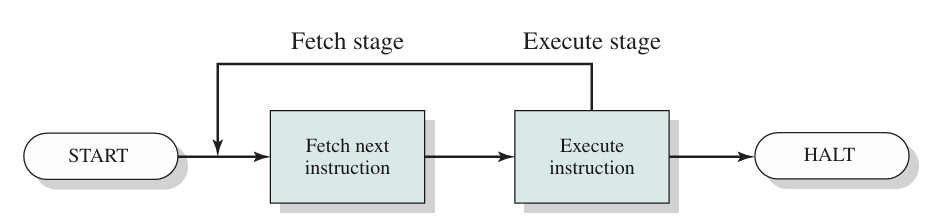
\includegraphics[width=0.7\textwidth]{figures/Ch01Figure2.png} % path to your figure
    \caption{\textbf{Fetch-Execute Cycle}}
    \label{fig:Ch01Fig2}
\end{figure}
At the beginning of each instruction cycle, the processor fetches an instruction
from memory. Typically, the program counter (PC) holds the address of the
next instruction to be fetched. Unless instructed otherwise, the processor always
increments the PC after each instruction fetch so it will fetch the next instruction
in sequence (i.e., the instruction located at the next higher memory address). For
example, consider a simplified computer in which each instruction occupies one 16-bit
word of memory. Assume that the program counter is set to location 300. The processor
will next fetch the instruction at location 300. On succeeding instruction cycles, it
will fetch instructions from locations 301, 302, 303, and so on. This sequence may be
altered, as explained subsequently.
The fetched instruction is loaded into the instruction register (IR). The instruction
contains bits that specify the action the processor is to take. The processor interprets
the instruction and performs the required action.

\vspace{0.5em}

Most modern processors include instructions that contain more than one address.
Thus, the execution stage for a particular instruction may involve more than one
reference to memory. Also, instead of memory references, an instruction may specify
an I/O operation.

\begin{methodbox}
\textbf{Instruction Execution Using the Fetch-Decode-Execute Cycle}

\begin{enumerate}
    \item \textbf{Fetch the instruction:}
    \begin{itemize}
        \item Read the instruction from the memory location pointed to by the PC into the IR.
        \item Increment the PC to point to the next instruction.
    \end{itemize} 
         
    \item \textbf{Decode the instruction:} 
    \begin{itemize}
        \item Examine the opcode in the IR to determine the operation to perform.
        \item Identify any operands or memory addresses involved.
    \end{itemize}  
    
    \item \textbf{Execute the instruction:} Perform the operation specified by the instruction:
    \begin{enumerate}
        \item For a load instruction, copy the contents from the specified memory address into the accumulator (AC).
        \item For an arithmetic instruction, perform the calculation using AC and memory contents.
        \item For a store instruction, write the contents of AC back to the specified memory address.
    \end{enumerate}
    
    \item \textbf{Repeat:} Return to the fetch step for the next instruction and continue until the program completes.
\end{enumerate}
\end{methodbox}

\subsubsection*{Unit 1.4: Interrupts}
\phantomsection
\addcontentsline{toc}{subsubsection}{Unit 1.4: Interrupts}
\bookmark[page=\thepage,level=3]{Interrupts}
An interrupt is a signal from a device or software indicating the need for attention or a request for a service. 
When an interrupt occurs, the processor temporarily halts its current activities, saves its state, and executes a function called an interrupt handler to deal with the event.
After the interrupt has been serviced, the processor resumes normal activities from where it left off.

The following table lists some common types of interrupts:
\begin{table}[h!]
\centering
\begin{tabular}{|l|p{10cm}|}  % p-column for better text wrapping
\hline
\textbf{Interrupt Type} & \textbf{Description} \\
\hline
Program & Generated by an error or exception in the program, such as division by zero or invalid memory access. \\
\hline
Timer & Generated by a timer within the processor to allow the operating system to perform periodic tasks. \\
\hline
I/O & Generated by an I/O device to signal the completion of an operation or to request service. \\
\hline
Hardware Failure & Generated by hardware malfunctions, such as power failures or memory errors. \\
\hline
\end{tabular}
\caption{Classes of Interrupts}
\label{tab:interrupts}
\end{table}

Interrupts improve the efficiency and responsiveness of a computer system by allowing it to handle 
asynchronous events and prioritise tasks effectively.

Consider these motivations:
\begin{itemize}
    \item I/O devices are much slower than the CPU and memory.
    \item Without interrupts, the CPU would have to wait for I/O operations to complete, wasting valuable processing time.
    \item With interrupts, the CPU can continue executing other instructions while waiting for I/O operations to finish.
    \item When an I/O operation completes, the device sends an interrupt signal to the CPU, 
    which temporarily halts its current activities to service the interrupt.
    \item This allows the CPU to efficiently manage multiple tasks and respond to events in a timely manner.
\end{itemize}

\newpage

Let us now compare program execution with and without interrupts.

\begin{examplebox}
\textbf{Program Execution Without Interrupts}

Study the figure which illustrates program execution without interrupts and the accompanying description.

\noindent\rule{\textwidth}{0.4pt}

\begin{minipage}{0.65\textwidth}


\textit{\underline{User Program}}
\begin{enumerate}
    \item Execute code segment 1 that does not involve I/O
    \item WRITE calls (pause user program and execute \\ \textit{I/O program} on processor)
    \item Execute code segment 2 that does not involve I/O
\end{enumerate}


\textit{\underline{I/O Program}}
\begin{enumerate}
    \item Segment 4 copies data to the write buffer
    \item I/O command prints the data on printer (processor is idle while waiting for I/O operation to complete)
    \item Segment 5 notifies user program about success or failure of WRITE operation
\end{enumerate}
\noindent\rule{\textwidth}{0.4pt}

\end{minipage}%
\hfill
\begin{minipage}{0.32\textwidth}
    \centering
    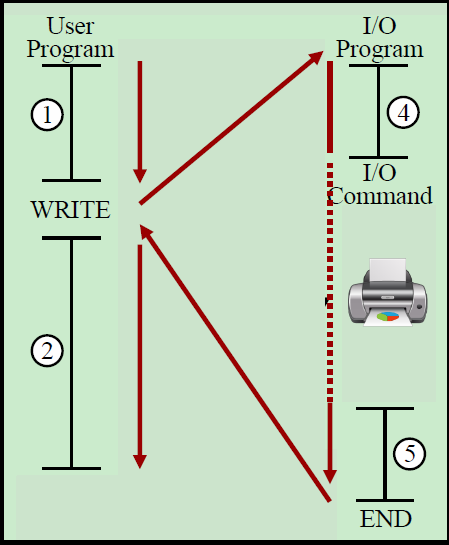
\includegraphics[width=\linewidth]{figures/Ch01Figure3.png}
    \captionof{figure}{\textbf{Execution without interrupts}}
    \label{fig:no_interrupts}
\end{minipage}

\vspace {0.5em}
Notice that without interrupts, the user program must wait until the I/O operation is complete before it can continue executing.
\end{examplebox}

\begin{examplebox}
    \textbf{Execution With Interrupts}

    Study the figure which illustrates program execution with interrupts and the accompanying \\ description.
    
    \noindent\rule{\textwidth}{0.4pt}
\begin{minipage}{0.65\textwidth}



\begin{enumerate}
    \item After \textbf{Segment 4}, the processor continues executing the \textbf{user program} (Segment 2) without waiting for the I/O to complete.
    \item The \textbf{I/O module} executes the I/O command independently, running in parallel with the user program.
    \item When the I/O operation finishes, the I/O module sends an \textbf{interrupt request} to the processor.
    \item The processor \textbf{temporarily suspends} the user program and switches to the \textbf{interrupt handler routine}.
    \item The interrupt handler (Segment 5) completes the I/O service, notifies the user program of the result, and the processor \textbf{resumes the user program} exactly where it was interrupted.
\end{enumerate}

\noindent\rule{\textwidth}{0.4pt}

\end{minipage}%
\hfill
\begin{minipage}{0.32\textwidth}
    \centering
    \includegraphics[width=\linewidth]{figures/CH01Figure4.png} % replace with your image
    \captionof{figure}{\textbf{Execution with \\ interrupts}}
    \label{fig:with_interrupts}
\end{minipage}

\vspace {0.5em}

The key advantage of using interrupts is that the processor can perform other tasks while waiting for I/O operations to complete,
thereby improving overall system efficiency and responsiveness.
Note that interrupts can occur at almost any time, so the state of the user program must be saved and restored correctly to ensure proper execution.
\end{examplebox}

To accommodate interrupts, an interrupt stage is added to the instruction cycle, as shown in the figure below.
\begin{figure}[!h]
    \centering
    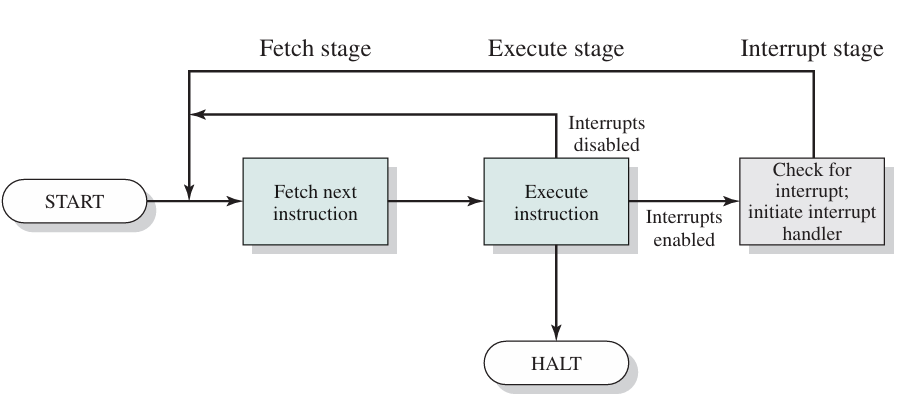
\includegraphics[width=0.7\textwidth]{figures/Ch01Figure5.png} % path to your figure
    \caption{\textbf{Instruction Cycle with Interrupts}}
    \label{fig:Ch01Fig5}
\end{figure}

To handle interrupts, the processor must perform several steps during the interrupt stage.
\begin{methodbox}
\textbf{Interrupt Handling by the Processor}

\begin{enumerate}
    \item \textbf{Save the status of the user program:} The processor stores the current state (registers, program counter, etc.) of the interrupted user program on the stack.
    \item \textbf{Set the Program Counter (PC):} The PC is updated to point to the start of the Interrupt Service Routine (ISR).
    \item \textbf{Execute the Interrupt Service Routine:} The processor executes the instructions in the ISR to handle the interrupt.
    \item \textbf{Restore the user program state:} After completing the ISR, the processor loads the saved state of the user program from the stack.
    \item \textbf{Resume user program execution:} The processor continues execution of the user program exactly where it was interrupted.
\end{enumerate}

\end{methodbox}

Naturally, this interrupt handling process introduces some overhead, as the processor must save and restore the program state.
However, the benefits of improved responsiveness and efficient multitasking generally outweigh this overhead.

\newpage

The following figure illustrates the changes in the memory and stack during interrupt handling.
\begin{figure}[!h]
    \centering
    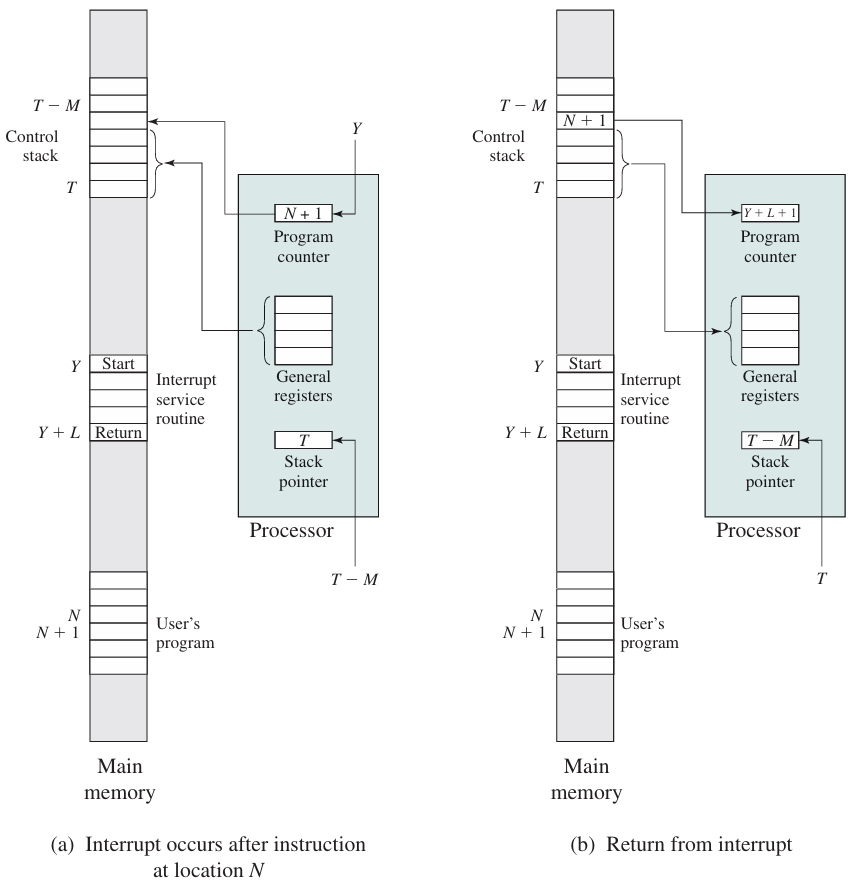
\includegraphics[width=0.7\textwidth]{figures/Ch01Figure6.png} % path to your figure
    \caption{\textbf{Memory and Stack Changes During Interrupt Handling}}
    \label{fig:Ch01Fig6}
\end{figure}

It is important to note that an interrupt may occur even while the processor is executing an interrupt handler.
For example, the computer may be receiving data from a keyboard while it is printing a document.

There are two common strategies to handle such nested interrupts:
\begin{itemize}
    \item \textbf{Sequential Interrupt Handling:} The processor completes the current interrupt handler before servicing any new interrupts. New interrupts are queued until the current handler finishes.
    \item \textbf{Priority-Based Interrupt Handling:} Each interrupt is assigned a priority level. If a higher-priority interrupt occurs while a lower-priority handler is executing, the processor temporarily suspends the lower-priority handler to service the higher-priority interrupt. After handling the higher-priority interrupt, the processor resumes the lower-priority handler.
\end{itemize}

\subsubsection*{Unit 1.5: The Memory Hierarchy}
\phantomsection
\addcontentsline{toc}{subsubsection}{Unit 1.5: The Memory Hierarchy}
\bookmark[page=\thepage,level=3]{The Memory Hierarchy}

The design constraints on memory can be reduced to three main factors: capacity, speed, and cost.
Considering capacity is a rather straight-forward issue. The more memory a computer has, the more programs and data it can store.

Speed, however, is a more complex issue. The speed of memory is usually measured in terms of access time, which is the time interval between the request for a word and the delivery of the word.
Memory access time must be considered in relation to the speed of the processor--it must keep up with the processor. If the memory is too slow, the processor will have to wait for it to deliver data, resulting in wasted processing time.

Cost is the final factor. The cost of memory is usually expressed in terms of cost per bit. The lower the cost per bit, the more memory can be provided within a given budget. The cost of memory must also be reasonable in relation to the cost of the other hardware components.
\newpage
As one might expect, there is a trade-off among these three factors:
\begin{itemize}
    \item Faster access time $\Rightarrow$ Higher cost per bit
    \item Larger capacity $\Rightarrow$ Lower cost per bit
    \item Larger capacity $\Rightarrow$ Slower access time
\end{itemize}

The solution to this trade-off is to use a memory hierarchy, which is a structure that uses multiple types of memory, each with different speeds, costs, and capacities.

\begin{figure}[!h]
    \centering
    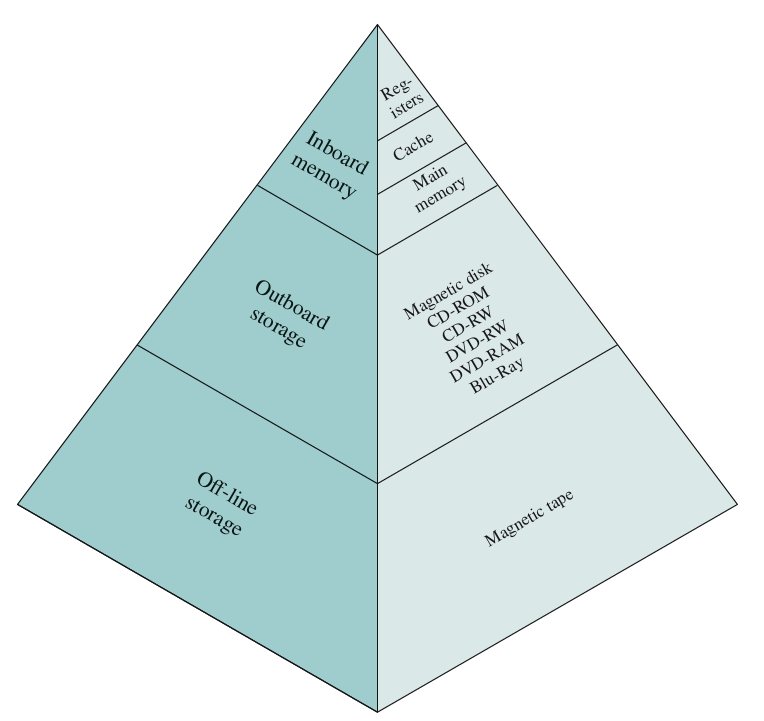
\includegraphics[width=0.7\textwidth]{figures/Ch01Figure7.png} % path to your figure
    \caption{\textbf{The Memory Hierarchy}}
    \label{fig:Ch01Fig7}
\end{figure}

Figure \ref{fig:Ch01Fig7} illustrates a typical memory hierarchy.
The trend, going from the top to the bottom of the hierarchy, is as follows:
\begin{itemize}
    \item Decreasing cost per bit
    \item Increasing capacity
    \item Increasing access time (i.e., slower speed)
    \item Decreasing frequency of access to memory by the processor
\end{itemize}

\begin{examplebox}
    \textbf{Two-Level Memory Hierarchy Example}

    A processor has access to two levels of memory:
    \begin{itemize}
        \item \textbf{Level 1 ($L_1$)}, with 1 000 bytes and an access time of 0.1 $\mu$s. (This is typically a cache memory.)
        \item \textbf{Level 2 ($L_2$)}, with 100 000 bytes and an access time of 1 $\mu$s. (This is typically the main memory.) 
    \end{itemize}

    Assume that if data is found in $L_1$, then the processor accesess it directly. (This is called a \textit{hit}.)
    If the data is found in $L_2$, then it is copied to $L_1$ and accessed from there. (This is called a \textit{miss}.)

    The average access time of the memory hierarchy can be calculated using the formula:
    \[
    \text{Average Access Time} = (h \times t_1) + \big((1 - h) \times (t_1 + t_2)\big)
    \]
    where:
    \begin{itemize}
        \item $h$ is the hit ratio (the fraction of accesses found in $L_1$),
        \item $t_1$ is the access time of $L_1$,
        \item $t_2$ is the access time of $L_2$.
    \end{itemize}


    Suppose that 95\% of the memory accesses are found in $L_1$ (i.e., $h = 0.95$). Then:
    \[
    \text{Average Access Time} = (0.95 \times 0.1 \mu s) + (0.05 \times \mu s + 1\mu s) = 0.095 \mu s + 0.05 \mu s = 0.15 \mu s.
    \]
\end{examplebox}

Now the big question is: How can we achieve a high hit ratio?
Observations show that memory accesess by the processor tend to cluster (loops, arrays, etc.). This is called the \textit{principle of locality}.

The solution is to organise data across the memory hierarchy so that data in such a way that the current cluster in use is in the fastest (the cache) memory.


\subsubsection*{Unit 1.6: Cache Memory}
\phantomsection
\addcontentsline{toc}{subsubsection}{Unit 1.6: Cache Memory}
\bookmark[page=\thepage,level=3]{Cache Memory}

Although cache memory is invisible to the OS, it interacts with other memory management components.

On all instruction cycles the processor accesess memory at least once to fetch the instruction and 
often more than once to fetch data. If the memory is slow, the processor will have to wait for it to deliver data, 
resulting in wasted processing time.

The solution to this problem is to exploit the principle of locality by providing a small, fast memory called \textit{cache memory} that holds the most frequently 
used instructions and data.

Cache principles are as follows:
\begin{itemize}
    \item The cache is smaller and faster than main memory.
    \item The cache is located between the processor and main memory.
    \item When the processor needs to read or write a location in main memory, it first checks whether that location is in the cache.
    \item If the location is in the cache (a \textit{hit}), the processor reads or writes the location in the cache.
    \item If the location is not in the cache (a \textit{miss}), the processor reads the location from main memory and also copies it to the cache.
    \item The cache is managed by hardware, which automatically handles the transfer of data between the cache and main memory.
\end{itemize}

Cache memory can be organised in several ways, but the most common is to divide the cache into blocks (clusters), where each block holds a fixed number of words.
The cache consists of slots that can hold one block each. If a word is not in the cache, an entire block containing that word is copied from main memory to the cache.
A binary tag is then added to identify each block in the cache.

\end{document}